\chapter{Results}

This chapter will present results from testing the landmark detector methods and the quality indicator on SSS data. The data was acquired in the Trondheims fjord by \textit{AURLab} using their vehicle \textit{LAUV Fridtjof} \cite{LAUVNTNU}. Fig. \ref{fig:neptus_screenshot} shows a map of parts of the Trondheim fjord and marks where the data was acquired. Further, the data was divided into a training and a test dataset. The training dataset was used to tune the landmark detectors, and the test set was used to evaluate the performance. 
\\
\\

\begin{figure} [h]% order of priority: h here, t top, b bottom, p page
  \centering
  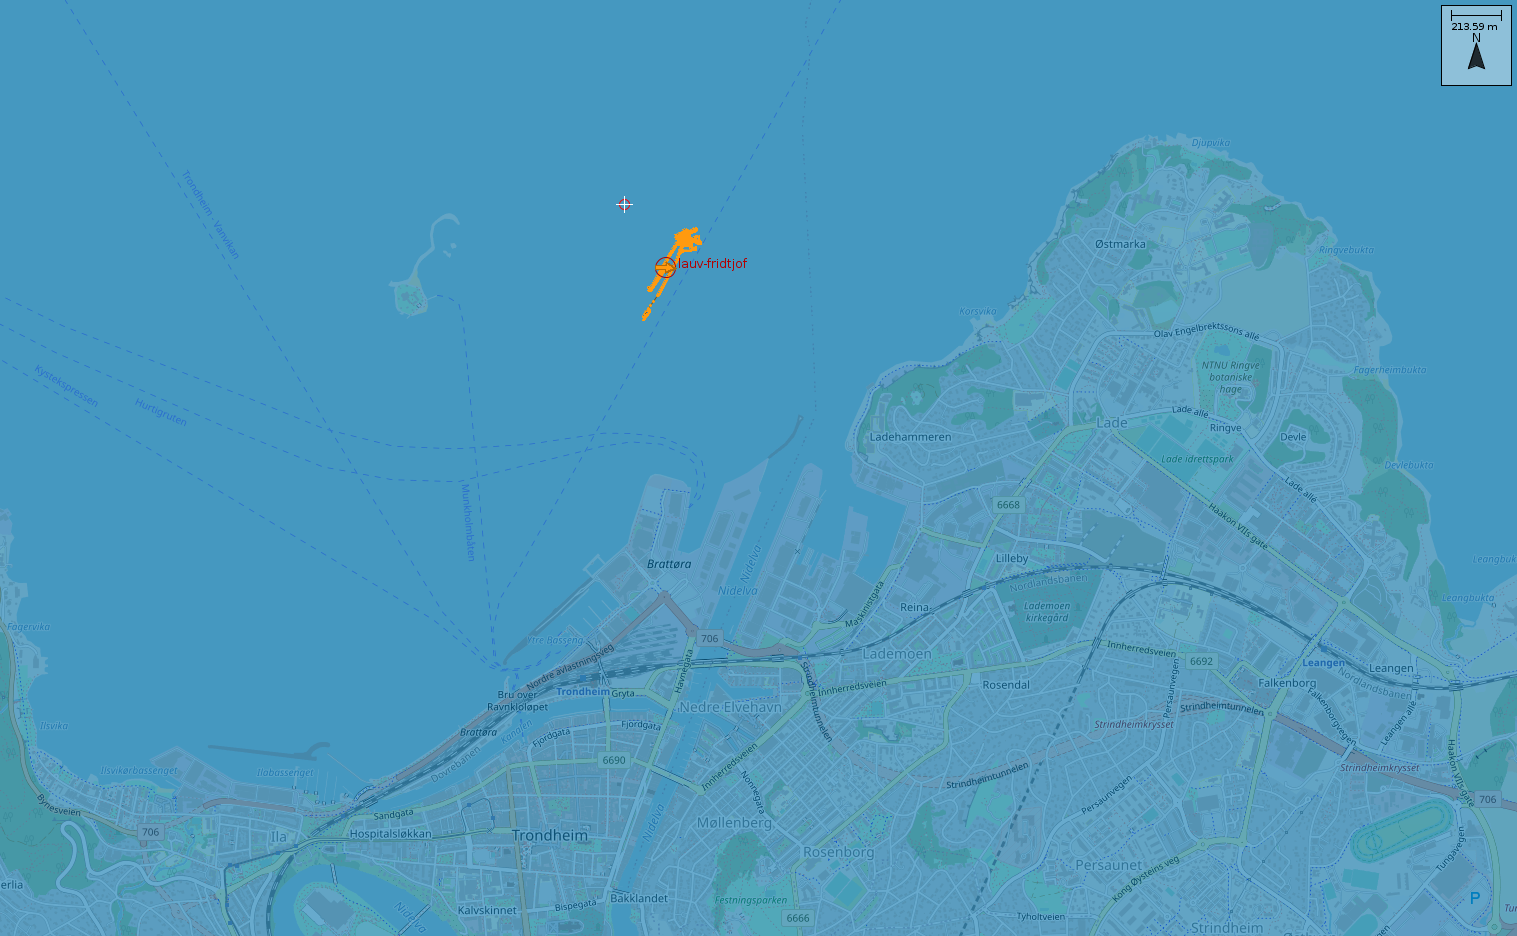
\includegraphics[width=0.9\textwidth]{figures/neptus_screenshot.png}
  \caption{Map showing part of the Trondheim fjord and where the data in this report was acquired.}
  \label{fig:neptus_screenshot}
\end{figure}

\section{Side scan sonar quality indicator}

The quality indicator is a measure that tries to say something about the quality of the SSS data, a measure that should be lower when turning due to overlapping swaths. Fig. \ref{fig:path_and_quality_ind} shows the result of testing the quality indicator. The left side is a plot of the path of the AUV in the xy-plane. Since the AUV is assumed to have an approximately constant altitude during the survey, altitude data is omitted. Further, the quality indicator is overlayed as the color of the path. As expected, the data quality decreases when turning due to swath overlapping. In addition, the traveled distance in the xy-plane is also shown along the path. The acquired sonar data traveling along the path is plotted on the right side, and the image's bar on the right side is the quality indicator. At a traveled distance of around $60 m$, two banana-like shadows appear. These could typically be examples of the anomalies and degradation of quality experienced when turning during a sonar survey. 

\begin{figure} % order of priority: h here, t top, b bottom, p page
  \centering
  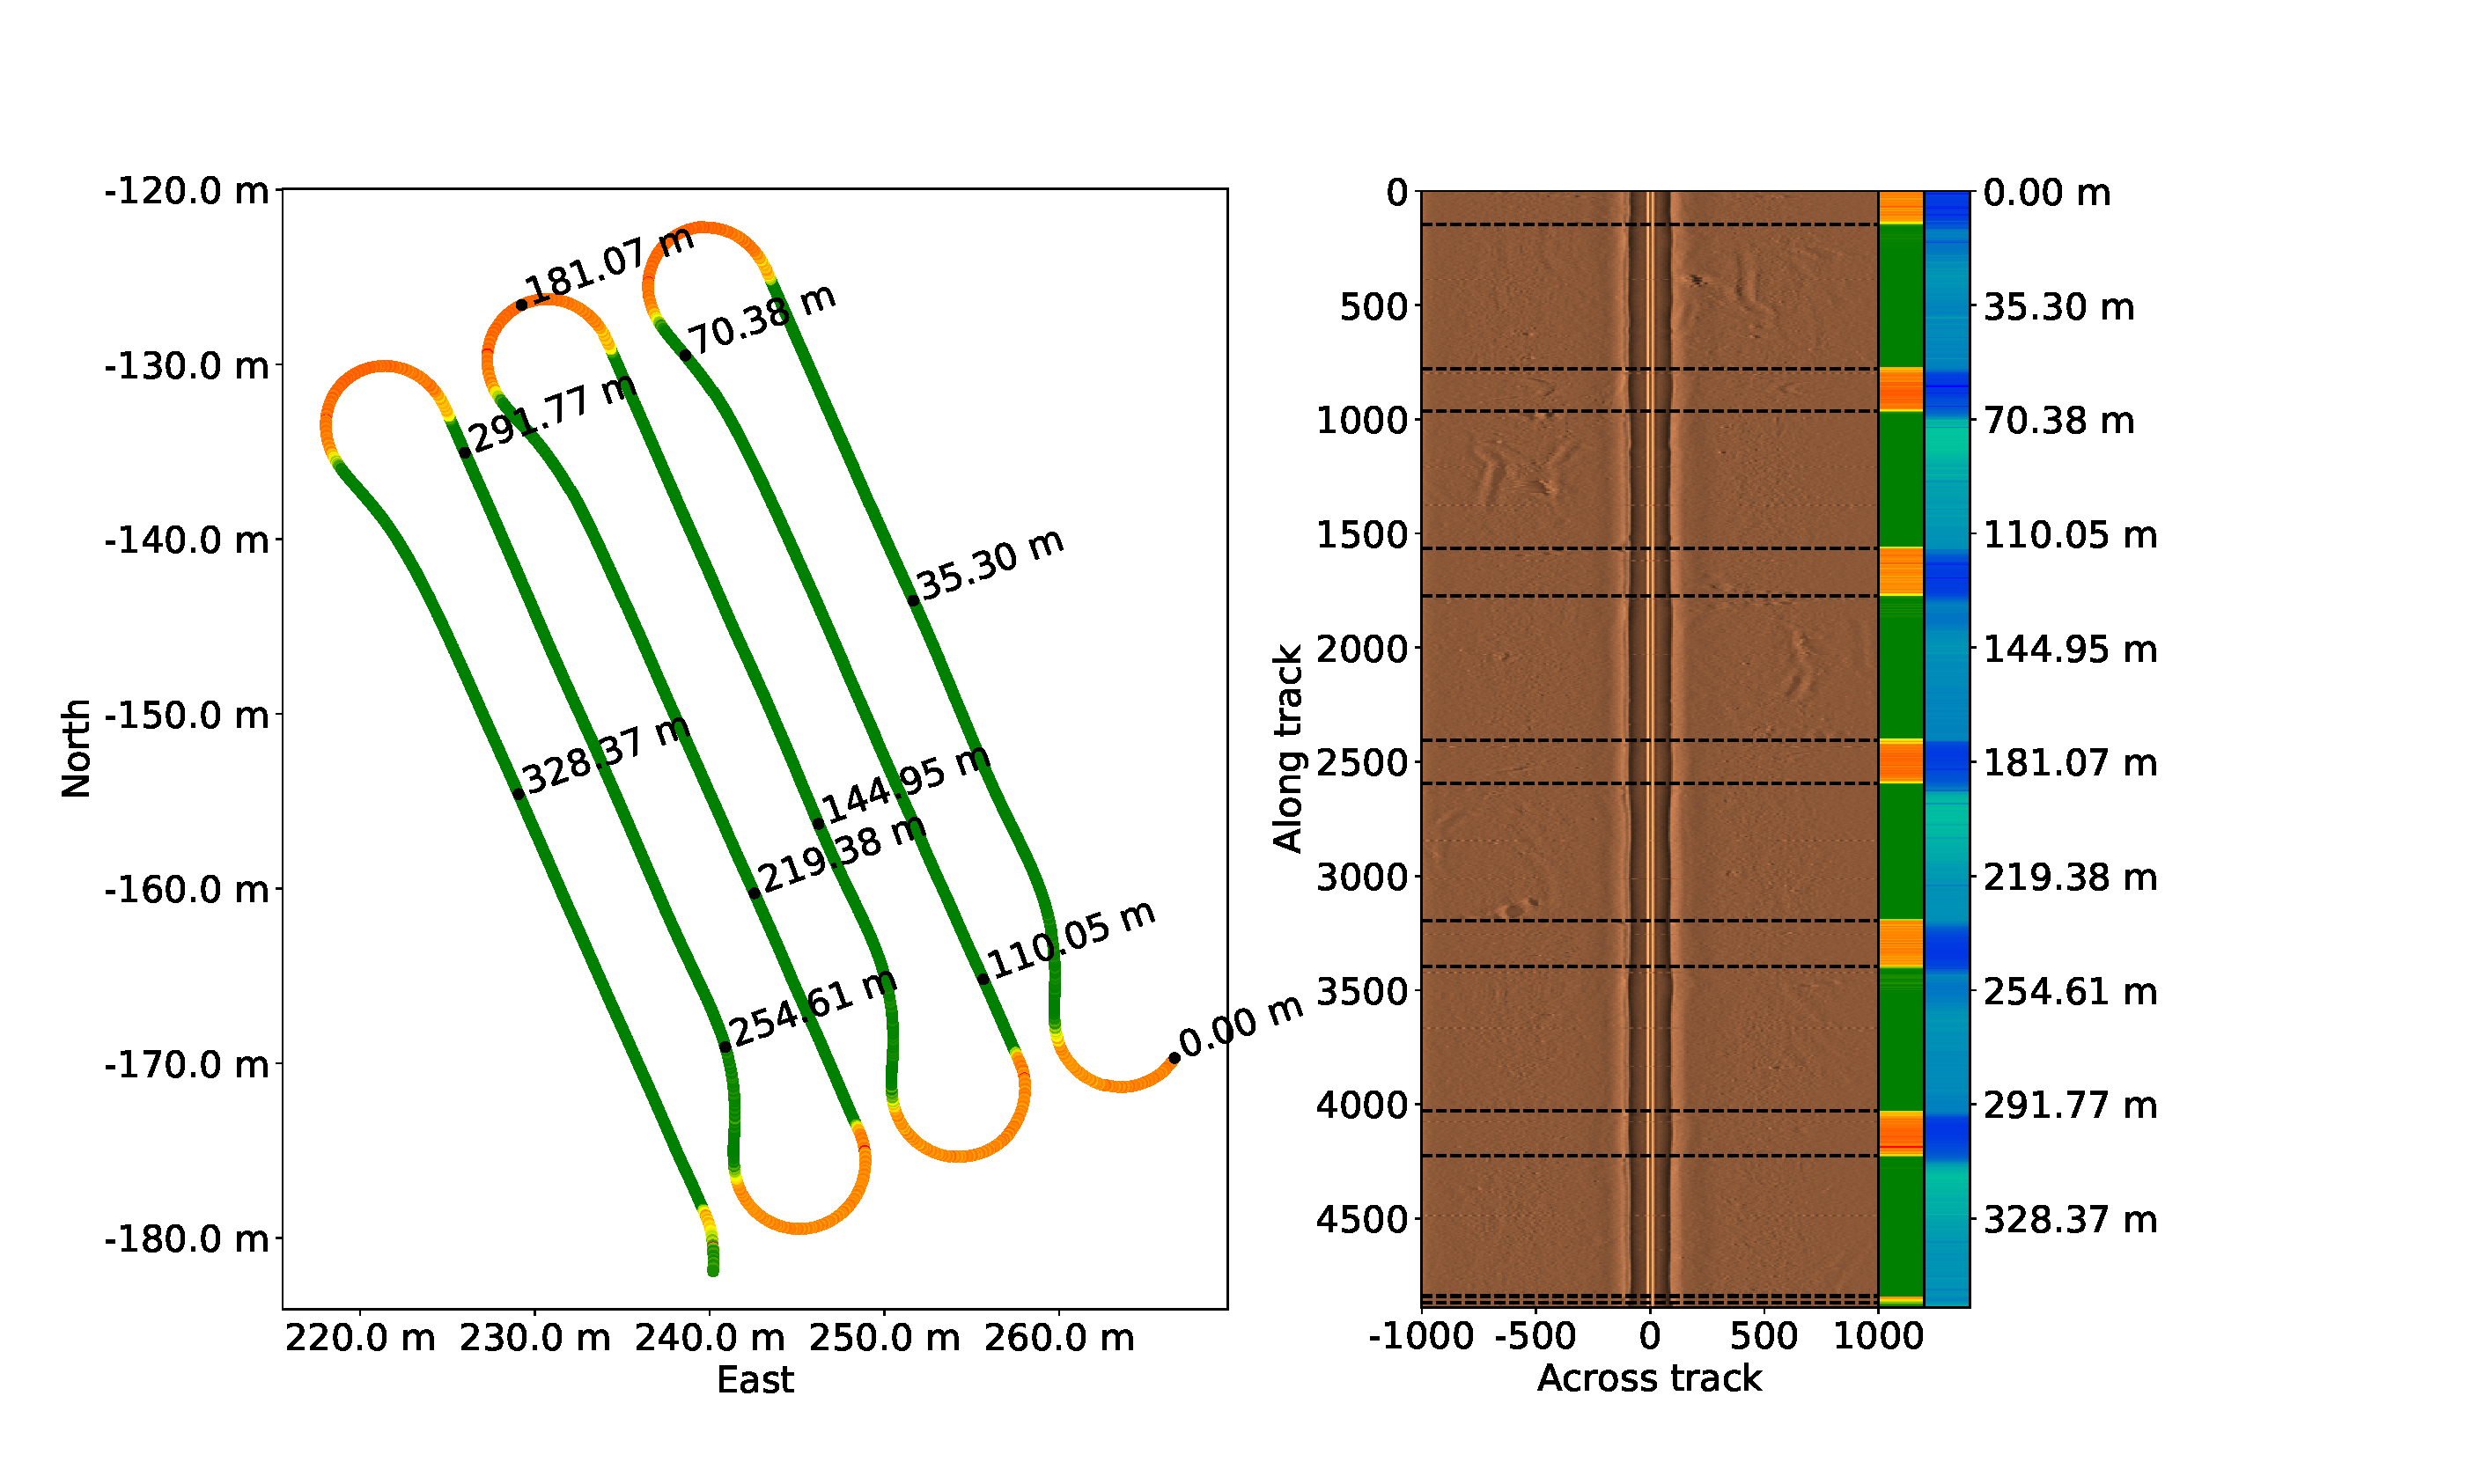
\includegraphics[width=1.0\textwidth]{figures/path_and_quality_indicator.eps}
  \caption[Path with quality indicator overlayed]{\textit{Left:} The traveled path in the xy-plane of the AUV. The path's color corresponds to the quality indicator along the path, and the traveled distance is also shown. \textit{Right:} The right figure shows the sonar image acquired from moving along the path and the corresponding quality indicator.}
  \label{fig:path_and_quality_ind}
\end{figure}

\section{1D Landmark Detector using Peak Detection}

The 1D landmark detector has four tuning parameters, the threshold $t$, smoothing parameter $s$, and the kernel size of the quadratic kernels used for the opening and closing operators. Fig.\ref{fig:1D_norm_tuning_training} shows the results from tuning, with three different thresholds represented. The middle threshold of $t = 1550$ was chosen. Even though there is not much difference between the different thresholds, there are some that make the selected threshold preferable over the other. For the threshold of $t = 1500$, an echo landmark on the left swath at around swath number $3100$ is missing compared to the chosen threshold. For $t = 1600$, two extra landmarks in the left swath around swath number $1000$ and $1200$ are detected. The landmark at swath number $1000$ is a real landmark. However, the detected landmark around swath number $1200$ is only partially detected and is therefore unwanted. A smoothing parameter of $s = \num{1e-5}$ was chosen to filter out enough noise not to get false positives. As the figure shows, there are not a lot of false positives, but to a cost of filtering out a large fraction of the details. To further filter the landmarks, the quadratic kernel used for the closing operation was chosen with a size of $10^2$, and the size of the kernel for the opening operation was chosen as $15^2$, such that the detected landmarks are both consistent and that narrow landmarks are removed, respectively.  

\begin{figure}  % order of priority: h here, t top, b bottom, p page
  \centering
  \includegraphics[width=1.0\textwidth]{figures/1D_norm_tuning_training.eps}
  \caption[Results of tuning threshold of the 1D method]{Results from tuning the thresholds of the 1D method with three different thresholds. Shadow landmarks are shown in green and echo landmarks are in purple. The rightmost bar on the right side is the vehicle's speed, where darker colors represent slower speeds. The second bar is the quality indicator.}
  % Parameters used: smoothing e-5, closing kernel (10,10), opening kernel (15,15)
  \label{fig:1D_norm_tuning_training}
\end{figure}


% \begin{figure}  % order of priority: h here, t top, b bottom, p page
%      \centering
%      \begin{subfigure}[b]{0.3\textwidth}
%          \centering
%          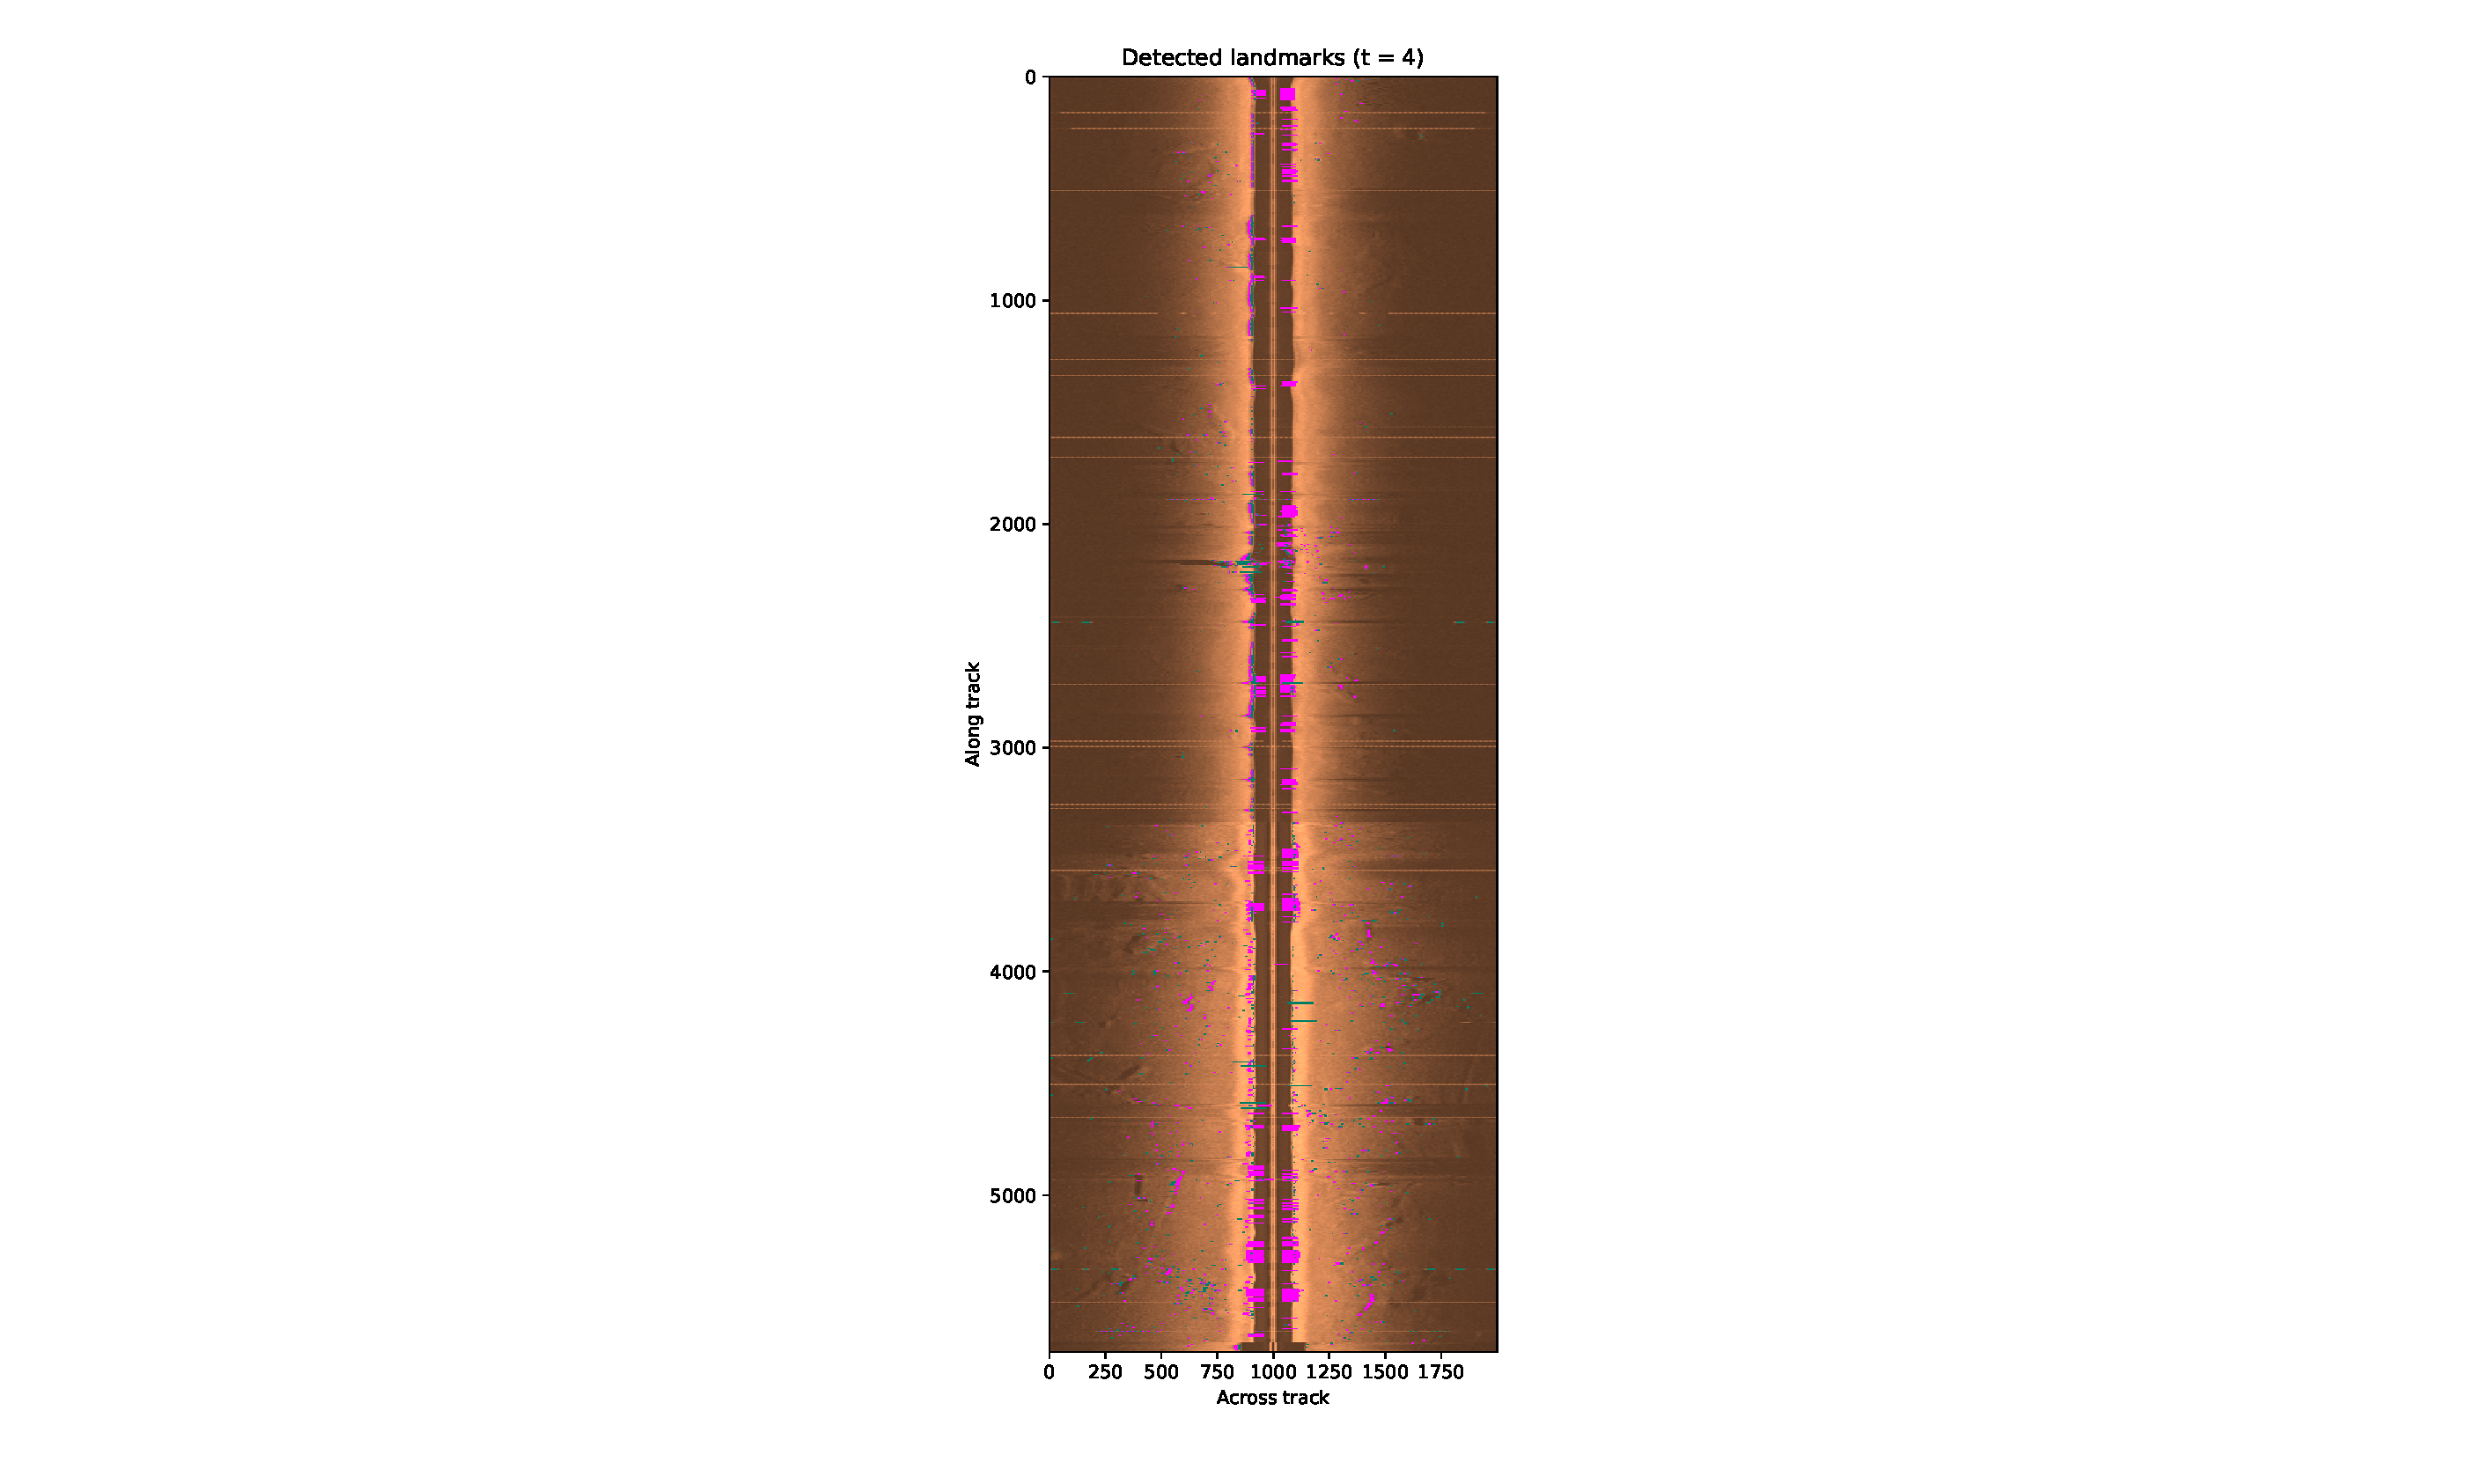
\includegraphics[trim=18cm 1cm 18cm 1cm, clip=true, width=\textwidth]{figures/1D_raw_tuning_t_4.eps}
%      \end{subfigure}
%      \hfill
%      \begin{subfigure}[b]{0.3\textwidth}
%          \centering
%          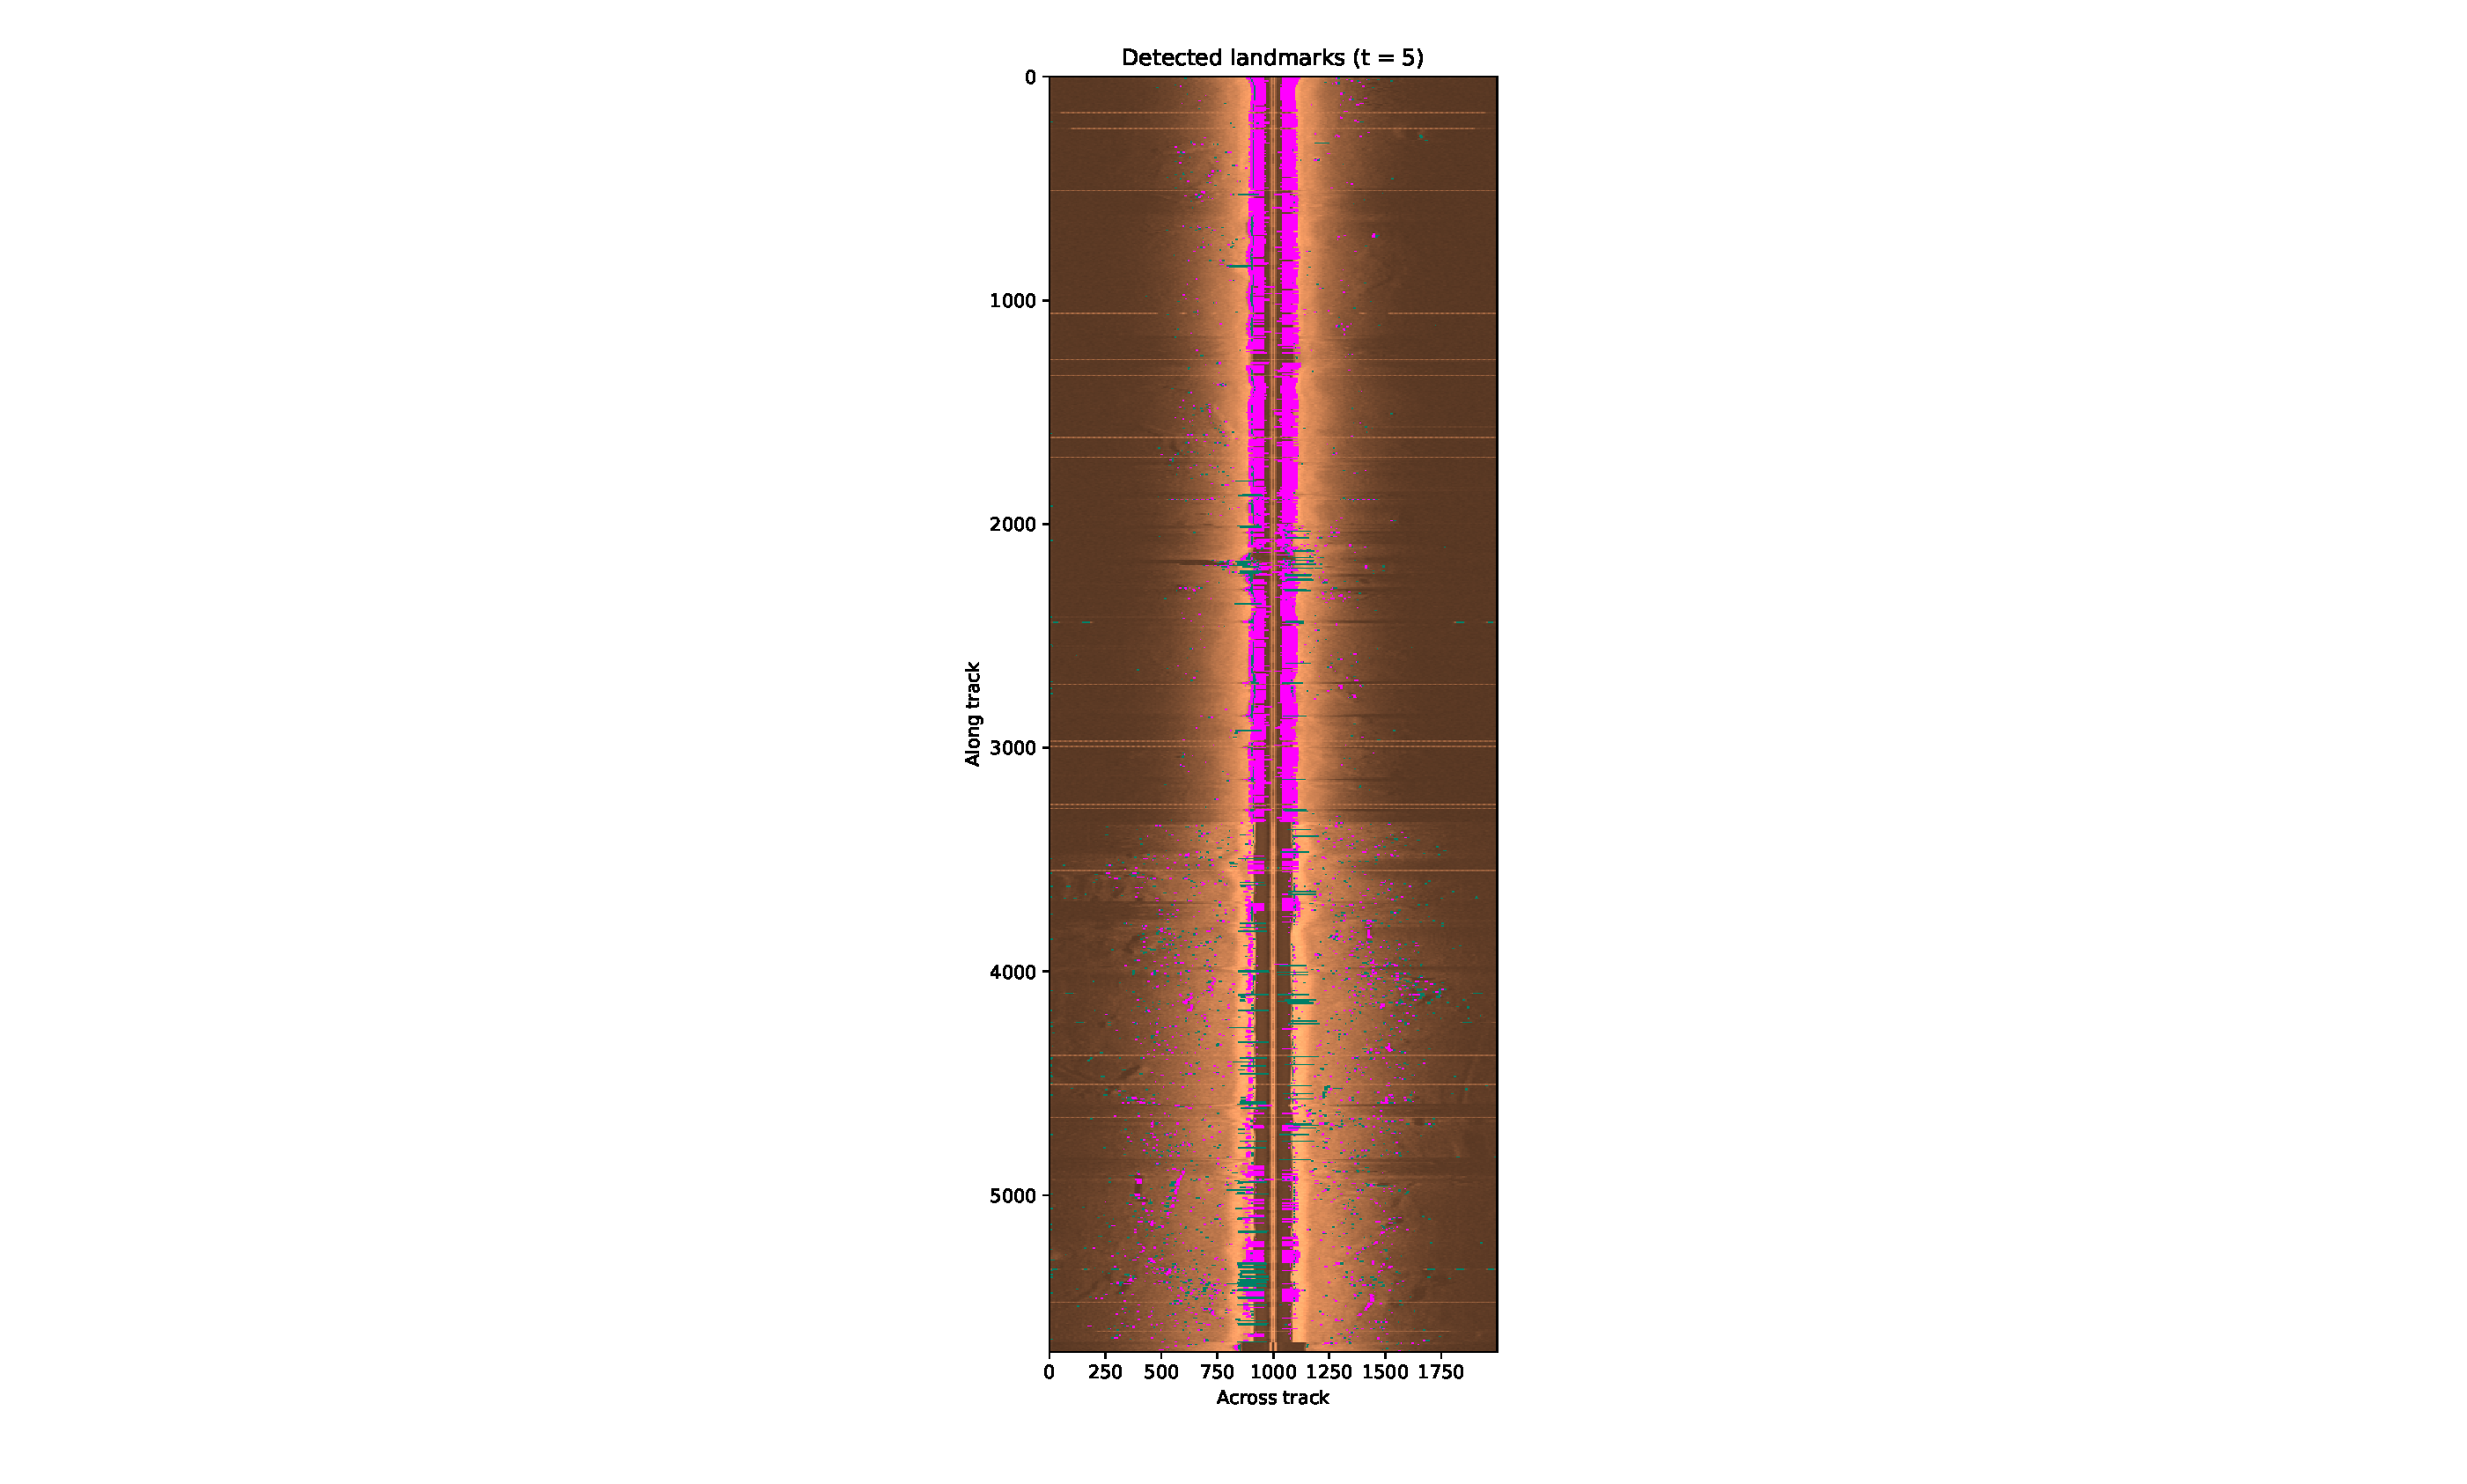
\includegraphics[trim=18cm 1cm 18cm 1cm, clip=true, width=\textwidth]{figures/1D_raw_tuning_t_5.eps}
%      \end{subfigure}
%      \hfill
%      \begin{subfigure}[b]{0.3\textwidth}
%          \centering
%          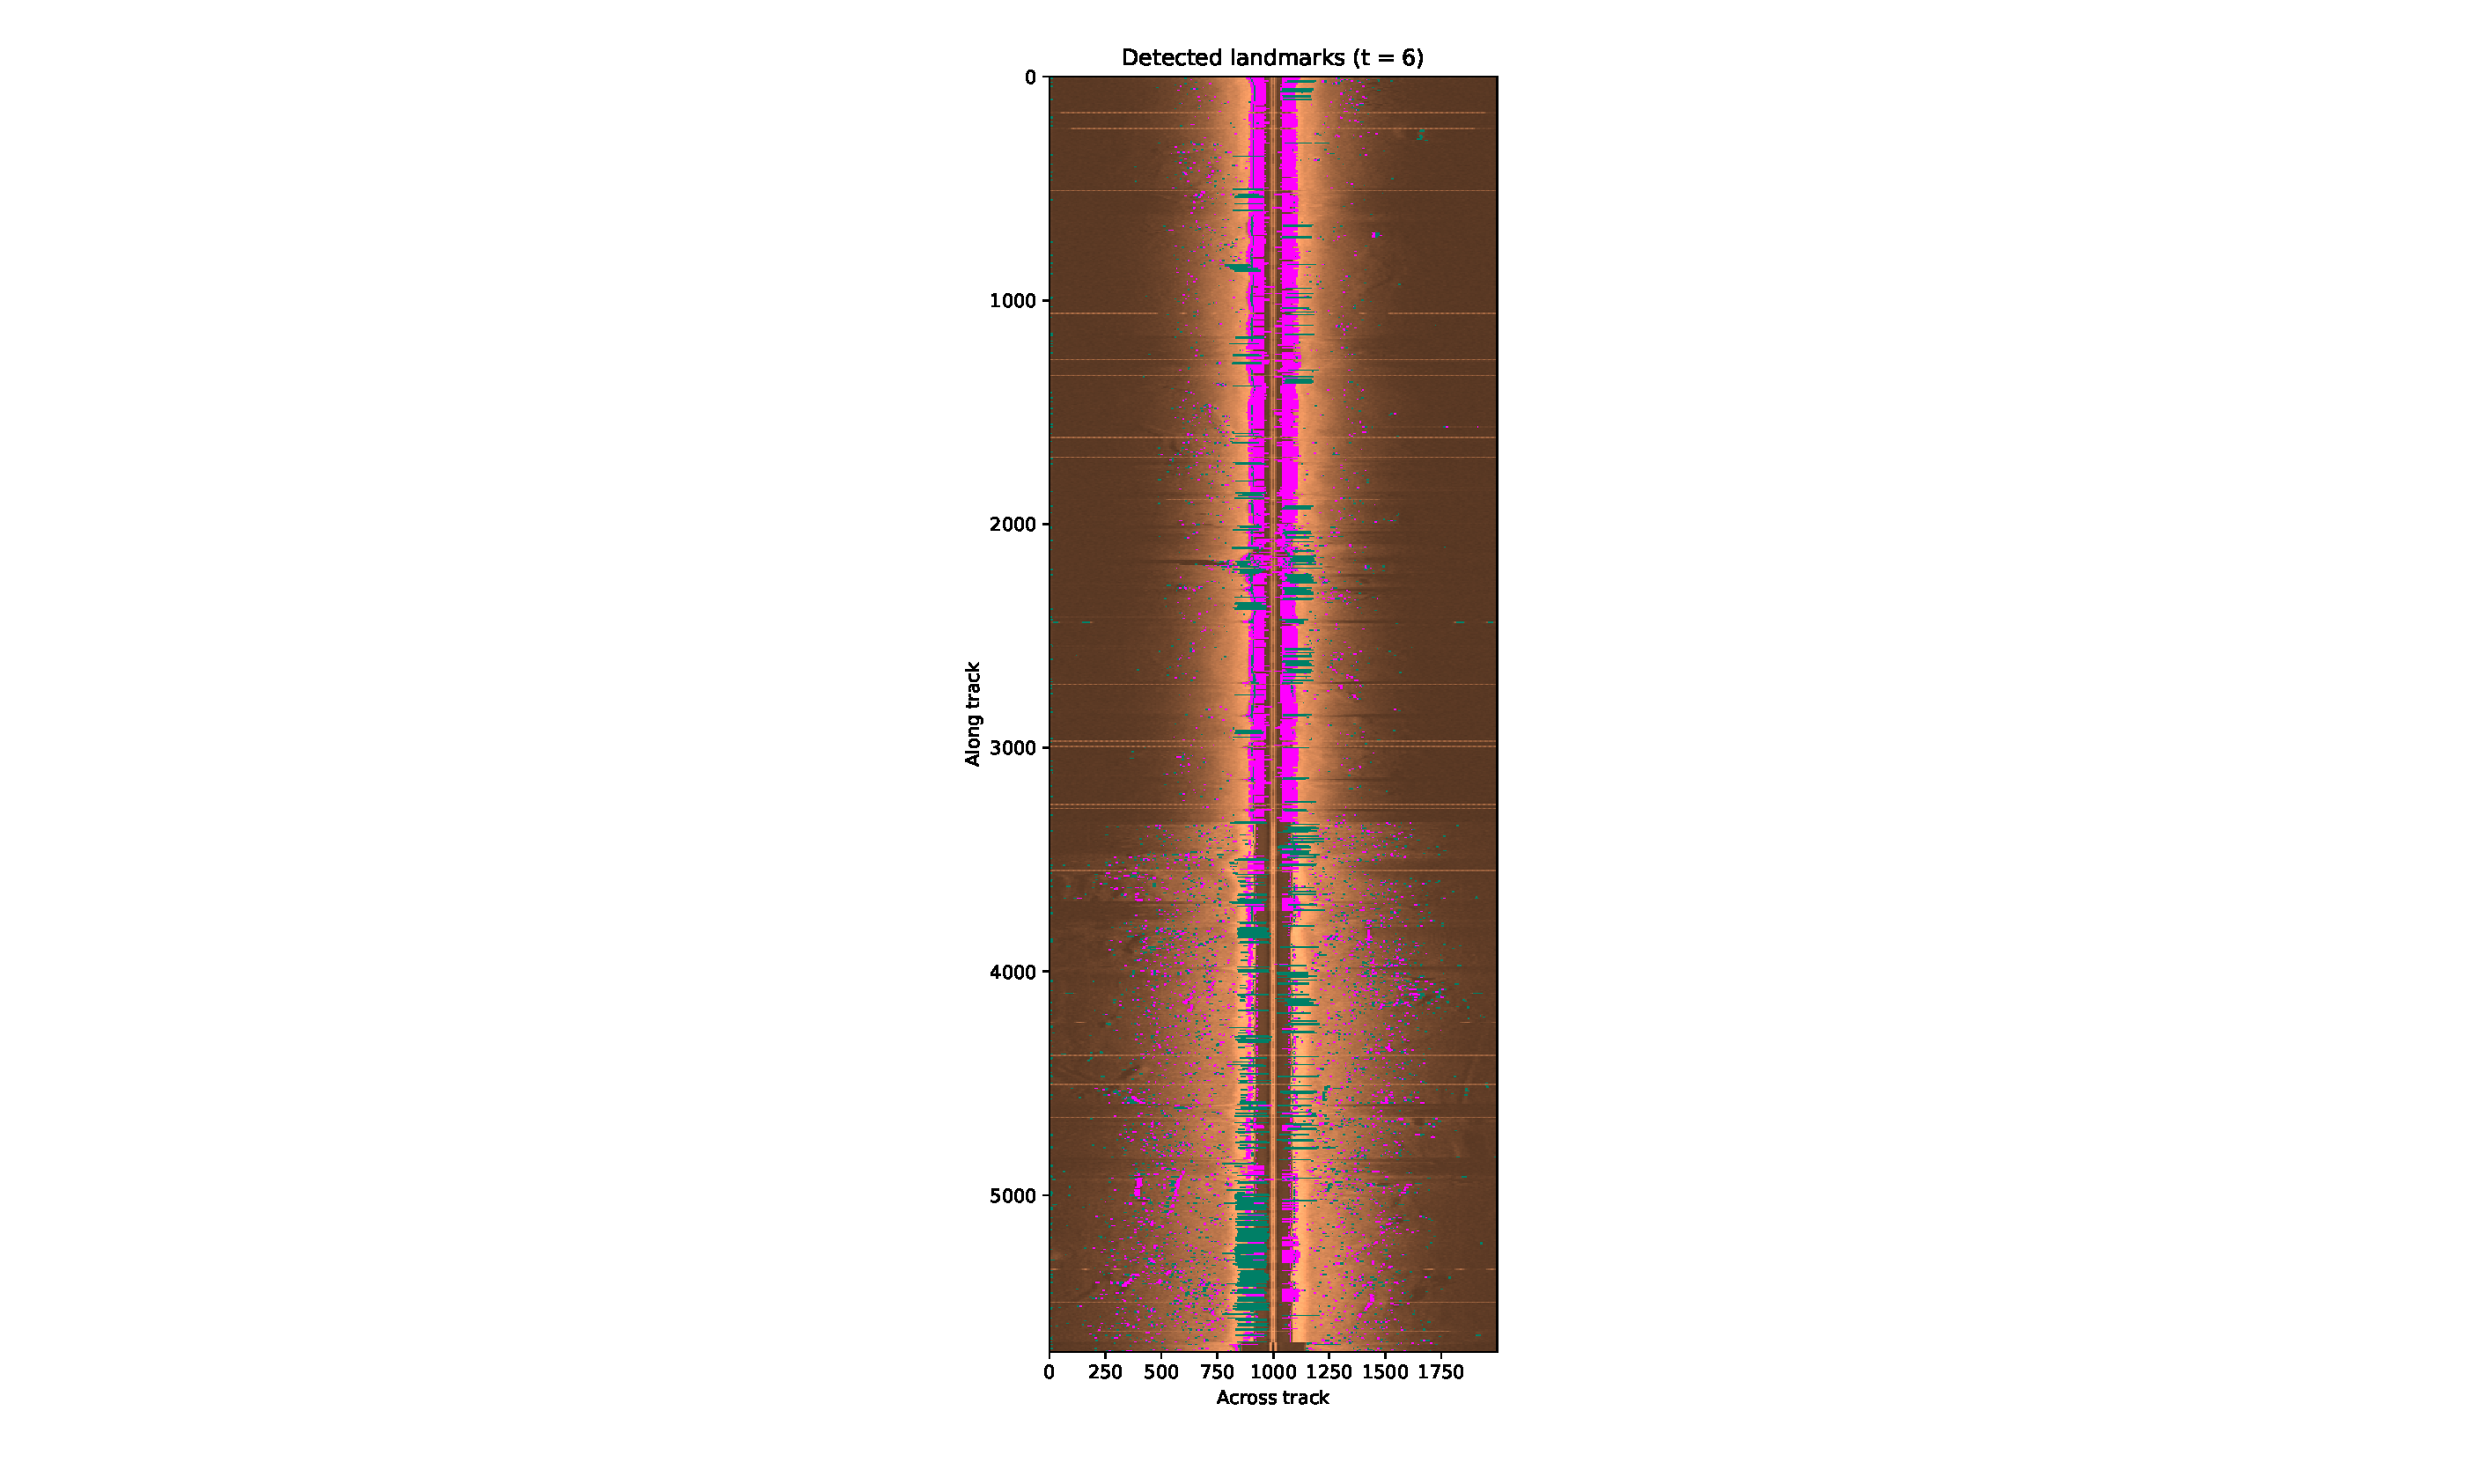
\includegraphics[trim=18cm 1cm 18cm 1cm, clip=true, width=\textwidth]{figures/1D_raw_tuning_t_6.eps}
%      \end{subfigure}
%         \caption{Results of tuning the 1D landmark detector method on raw data}
%         \label{fig:1D_raw_tuning}
% \end{figure}

\section{2D Landmark Detector using Expert Rules}

The 2D landmark detector has a total of six parameters to tune. The parameter $d_{ob min}$ was set to $3 m $, as in \cite{Leblond2019SonarProject}. Fig. \ref{fig:2D_tuning_intensity_thres} shows the result from tuning the intensity threshold with three different intensity thresholds displayed. The intensity threshold of $t_i = 0.85$ was chosen. An intensity threshold of $t_i = 0.8$ results in few false positives or noise in the detected landmark candidates. However, landmark candidates without a strong shadow are not detected consistently. Several large landmark candidates either have holes or are not consistently detected. An intensity threshold of $t_i = 0.9$ results in much more noise in the detected landmark candidates, which is unwanted. An intensity threshold of $t_i = 0.85$ produces consistent landmark candidates and an acceptable amount of noise. 

\begin{figure}  % order of priority: h here, t top, b bottom, p page
  \centering
  \includegraphics[width=1.0\textwidth]{figures/2D_tuning_threshold_training.eps}
  \caption[Results of tuning intensity threshold the 2D method]{Results from tuning the intensity threshold of the 2D method. The bar on the right side shows the speed of the AUV. The bar inside the speed shows the quality indicator. }
  \label{fig:2D_tuning_intensity_thres}
\end{figure}

Fig. \ref{fig:2d_tuning_paramaters_training} shows the results of tuning the last four parameters. The green landmark candidates are the landmarks filtered out in the corresponding step of the pipeline, and the purple landmarks are the kept landmarks. The leftmost image shows the sonar image. The second leftmost image results from filtering landmark candidates by along-track height. The landmark candidates are generated by applying intensity thresholding on the sonar image. Large landmarks are chosen to be filtered out because it is more difficult to detect them consistently, and therefore a more conservative choice is made. In addition, this step filters out much of the noise in the landmark candidates. The third image shows the result of applying the landmark area filtering. The parameter $A_{min} = 100$ was chosen to filter out the smallest landmarks. The fourth image shows the result of filtering out landmarks based on their fill rate of the rectangular bounding box encapsulating them. The fill rate limit was set to $r_{fr} = 0.3$ to filter out the thin and non-consistent landmarks. The last image shows the resulting landmarks.

\newpage

\begin{figure} [h!] % order of priority: h here, t top, b bottom, p page
     \centering
     \begin{subfigure}[bh]{0.59\textwidth}
         \centering
         \includegraphics[trim=0cm 3cm 0cm 2.8cm, clip=true, angle=90, width=0.85\textwidth]{figures/2D_tuning_parameters_training.eps}
         \caption[Results of tuning the geometrical thresholds 2D method]{Results from tuning the geometrical parameters of the 2D method on training data}
         \label{fig:2d_tuning_paramaters_training}
     \end{subfigure}
     \hfill
     \begin{subfigure}[bh]{0.395\textwidth}
         \centering
         \includegraphics[trim=0cm 6.6cm 0cm 6.5cm, clip=true, angle=90, width=0.85\textwidth]{figures/2D_result_test.eps}
         \caption[Results from testing the 2D landmark detector]{Results from running the 2D landmark detector on the test data}
         \label{fig:2d_result_test}
     \end{subfigure}
     \caption{The 2D landmark detector pipeline on training and test data. The purple landmarks are the kept landmarks in the corresponding step in the pipeline, and the green landmarks are filtered out.}
\end{figure}

\newpage

\section{Landmark detection on test data}

Both landmark detector methods were run on the test dataset to evaluate the performance of the landmark detectors with the chosen tuning parameters. Fig. \ref{fig:test_data} shows the test data. The result from the 1D landmark detector is shown in fig. \ref{fig:1D_norm_result_test}. No false positives are detected; however, several landmarks are only partially detected. It is also worth noting that only one echo landmark is detected. Fig. \ref{fig:2D_result_single_test} shows the result from the 2D landmark detector. The conservative tuning is evident in the result, as several large, thin landmarks at the top of the image are not detected. Further, the thin landmarks that are detected are only partially detected. 

\begin{figure} % order of priority: h here, t top, b bottom, p page
     \centering
    \begin{subfigure}[t]{0.66\textwidth}
         \centering
         \includegraphics[trim=5cm 0cm 7cm 1.2cm, clip=true, width=\textwidth]{figures/test_data_plain.eps}
         \caption{Test data}
         \label{fig:test_data}
     \end{subfigure}
     \hfill
     \begin{subfigure}[b]{0.45\textwidth}
         \centering
         \includegraphics[trim=11cm 0cm 13cm 0cm, clip=true, width=\textwidth]{figures/1D_norm_result_test.eps}
         \caption{1D landmark detector. Green is echo landmarks, and purple is shadow landmarks.}
         \label{fig:1D_norm_result_test}
     \end{subfigure}
     \hfill
     \begin{subfigure}[b]{0.45\textwidth}
         \centering
         \includegraphics[trim=11cm 0cm 13cm 0cm, clip=true, width=\textwidth]{figures/2D_result_single_test.eps}
         \caption{2D landmark detector. Purple is the detected landmarks}
         \label{fig:2D_result_single_test}
     \end{subfigure}
        \caption{Results from running landmark detectors on test data}
        \label{fig:landmark_detection_test_data}
\end{figure}
